\section{Event reconstruction and particle identification}
%%%%%%%%%%%%%%%%%%%%%%%%%%%%%%%%%%%%%%%%%%%%%%%%%%%%%%
\label{sec:Objects}

In CMS, the physics object reconstruction and identification is based on standard algorithms developed by the collaboration and used by all the physics analyses. In this section, the techniques used for the reconstruction and identification of the physics objects of interest for \hwwllnn analyses are described.

\subsection{The Particle Flow technique}\label{sec:PF}

The Particle Flow (PF) event reconstruction technique~\cite{CMS-PAS-PFT-09-001} aims at the reconstruction and identification of all the stable particles in the event, i.e. electrons, muons, photons, charged and neutral hadrons, with a thorough combination of the information from all CMS sub-detectors, in order to determine their energy, direction and type. These individual particles are then used, for example, to build jets, to measure the missing transverse energy \MET, to reconstruct the $\tau$ from their decay products, to quantify the charged lepton isolation and to tag b-jets.

The CMS detector is well suited for this purpose. Indeed, the presence of a large internal silicon tracker immersed in an intense solenoidal magnetic field allows the reconstruction of charged particles with high efficiency and small fake rate, and provides a high precision measurement of the particle \pt down to about $150\,\MeV$, for $|\eta|\leq2.6$. The high granularity of the ECAL calorimeter is the additional key element for the feasibility of the PF technique, allowing the reconstruction of photons and electrons with high energy resolution.

The first step of the PF technique consists in the reconstruction of the basic elements from the various sub-detectors, such as charged-particle tracks, calorimeter clusters and muon tracks. These elements, which are provided by the sub-detectors with high efficiency an low fake rate, are then connected together with a link algorithm.

The good performance of the tracking system are achieved by means of an iterative tracking strategy~\cite{Chatrchyan:2014fea}, based on the Kalman Filter algorithm~\cite{Billoir:1990we}. The basic idea of iterative tracking is that initial iterations search for tracks that are easiest to find, e.g. high \pt tracks produced near the interaction region. After each iteration, hits associated to reconstructed tracks are removed from the hit collection, thereby reducing the combinatorial complexity and simplifying the subsequent iterations, which aim at finding more complicated set of tracks, e.g. low \pt or displaced tracks. The \emph{Iteration 0}, where the majority of tracks are reconstructed, is designed to identify prompt tracks with $\pt>0.8$\,\GeV that have three hits in the three layers of the pixel detector. \emph{Iteration 1} is used to recover prompt tracks that have only two pixel hits. \emph{Iteration 2} aims at finding low-\pt prompt tracks while \emph{Iterations 3--5} are intended to find tracks that originate outside the collision point, i.e. tracks produced by a secondary vertex, and to recover undetected tracks in the previous iterations. Each iteration proceeds according to four steps:
\begin{itemize}
\item \emph{seeding}: initial track candidates are obtained using 2 or 3 hits in the innermost layers (these proto-tracks are called seeds);
\item \emph{pattern recognition}: this step is based on Kalman Filter and searches for hits in the outer layers that could be associated to the initial track candidate, reconstructing the particle trajectory;
\item \emph{track fitting}: in this step a fit of the trajectory is performed, using its associated hits and providing an estimate of the track parameters (\pt, $\eta$, $\phi$, charge, etc.);
\item \emph{selection}: finally tracks are selected based on quality requirements.
\end{itemize}

The high detection efficiency of the calorimeters is based on a specific calorimeter clustering algorithm, which is performed separately in each sub-detector. The algorithm is based on three steps: in the first step, ``cluster seeds'' are identified as local calorimeter cells with an energy deposit above a given threshold. Then, ``topological clusters'' are grown from the seeds by gathering cells with at least one side in common with a cell already in the cluster, and with an energy above a given threshold. A topological cluster usually gives rise to many ``particle flow clusters'' as seeds, which are identified sharing the energy of each cell among the particle flow clusters, thereby allowing the determination of the particle flow cluster energy and position.

These elements are then connected to each other using a link algorithm, which identifies blocks of elements that are topologically compatible. For example, a charged-particle track is linked to a calorimeter particle flow cluster if the extrapolated position from the track to the calorimeter is compatible with the cluster boundaries. From these blocks, PF candidates are identified according to the following order:
\begin{itemize}
\item Muons: a \emph{global muon} gives rise to a \emph{PF muon} if its combined \pt measurement is compatible within 3 standard deviation with the one provided by the sole tracker. The corresponding track is removed from the block;
\item Electrons: electrons tend to give rise to short tracks, and to lose energy by Bremsstrahlung in the tracker layers on their way to the calorimeter. The link between a charged-particle track (refitted with the Gaussian-Sum Filter (GSF)~\cite{Adam:815410}) and one or more ECAL clusters identifies a \emph{PF electron}. After the identification, the corresponding tracks and clusters are removed from the block.
\item Charged hadrons: the remaining tracks give rise to \emph{PF charged hadrons}. Tracks can be linked to ECAL and HCAL clusters, and the energy is determined taking into account information from calorimeters;
\item Photons and neutral hadrons: ECAL clusters not linked with tracks give rise to \emph{PF photons}, while the remaining HCAL clusters are identified as \emph{PF neutral hadrons}.
\end{itemize}
After the identification of all PF candidates in the event, \emph{PF jets} are clustered as described in Sec.~\ref{chap2:jets}. The last step is the reconstruction of the \emph{PF \ptmiss}, which is given by:

\begin{equation} 
\ptmiss = - \sum_{\mathrm{PF\,obj}} \vec{p}_\mathrm{T}^\mathrm{\,PF\,obj} \quad,
\end{equation}

where the sum extends over all the PF objects. The \MET is defined as the modulus of \ptmiss.

\subsection{Leptons reconstruction and identification}

\subsubsection{Muon reconstruction and identification}
Muons produced at the collision point can go through the entire detector with a negligible energy loss, thus reaching the detector outermost part where the muon chambers are installed (see Sec.~\ref{sec:muonsyst}). Muons interact through ionization with the layers of the silicon tracker, which is able to reconstruct their tracks (\emph{tracker track}). The muon tracks are also reconstructed using the muon system (\emph{standalone muon track}). Based on these objects, two reconstruction approaches are used~\cite{Chatrchyan:2012xi}: in the first method (outside-in), for each standalone muon tracks a tracker track is searched for by extrapolating the two tracks to a common surface. If a match is found, the hits associated to the two tracks are fitted together giving rise to a \emph{Global Muon}. The second approach (inside-out) consists in considering all tracker tracks with $\pt > 0.5$\,\GeV as potential muon candidates and are extrapolated to the muon system taking into account the magnetic field, the expected energy losses and the multiple scattering in the detector material. If at least one muon segment (a short track stub made of DT or CSC hits) matches the extrapolated tracks, the corresponding tracker track is identified as a \emph{Tracker Muon}.

The matching with the muon system improves significantly the muon \pt resolution that can be obtained from the tracker only, especially in the region with $\pt > 200$\GeV, as shown in Fig.~\ref{fig:muptres}. 
\begin{figure}[htb]
\centering
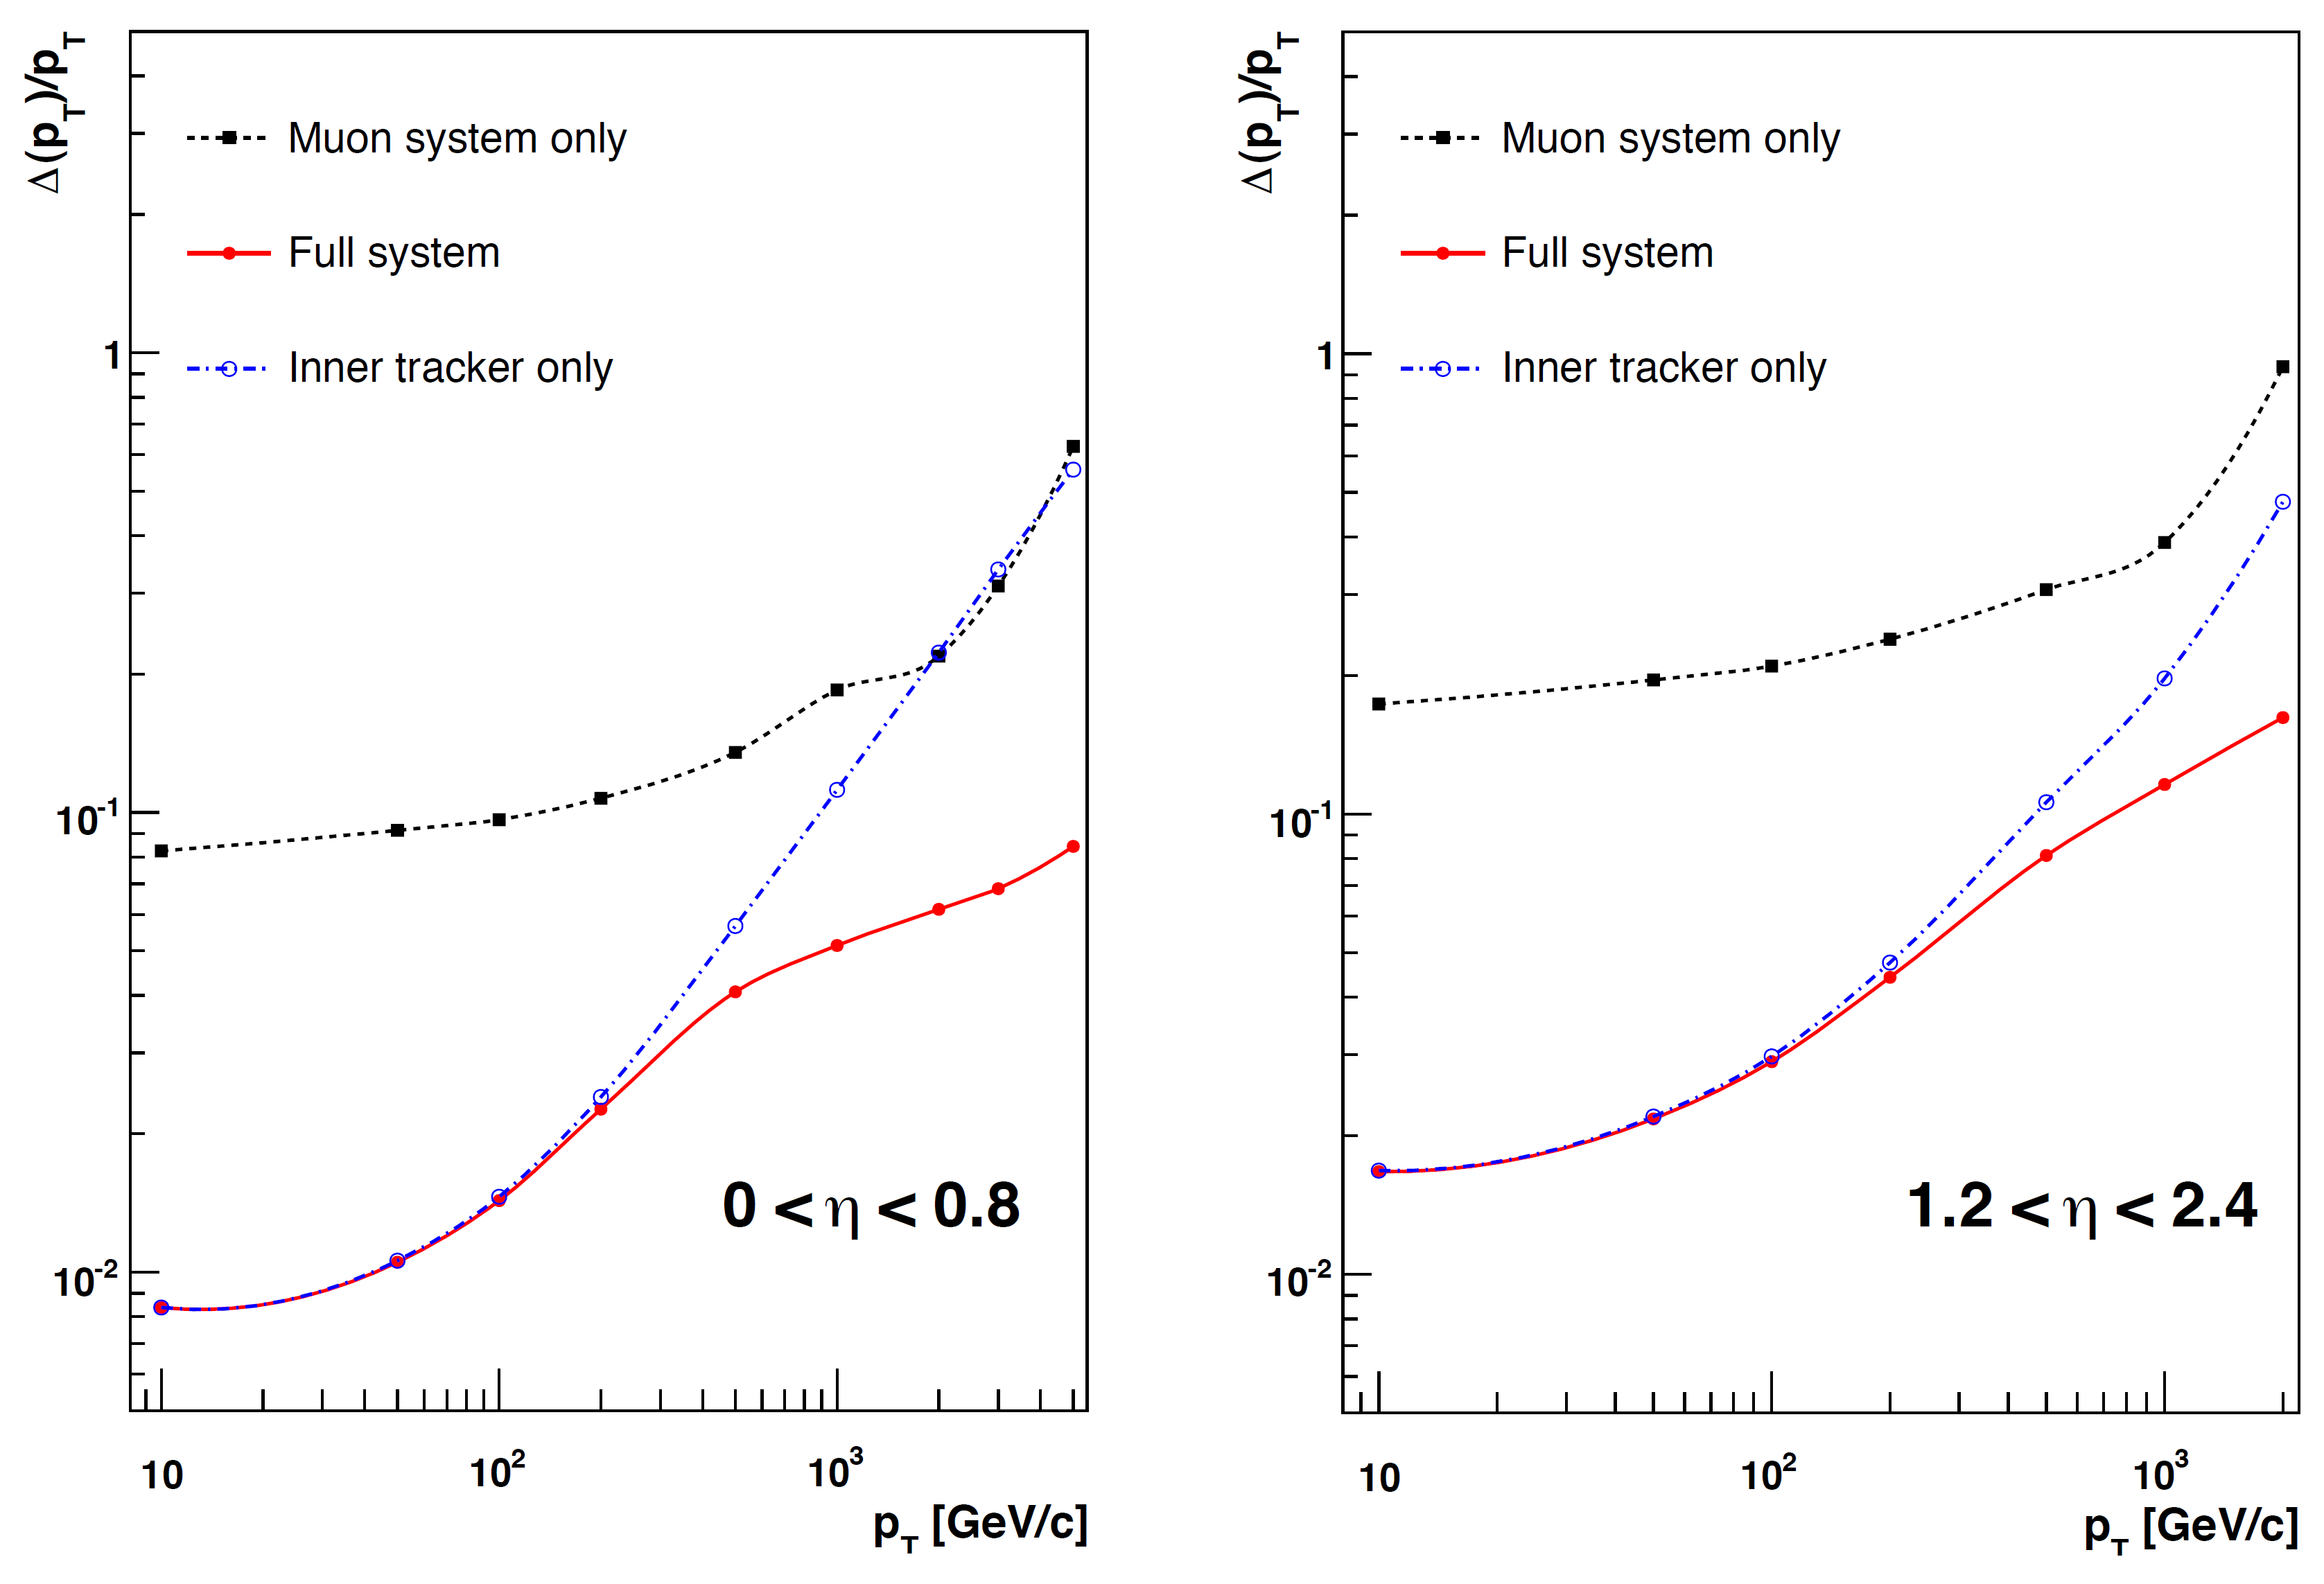
\includegraphics[width=0.6\textwidth]{images/muptres.png}
\caption{Muon \pt resolution as a function of the muon \pt in the barrel (left) and in the endcap (right) regions. The resolution is provided for the measurement using the tracking system or the muon system only, as well as for the combination of the two methods.}\label{fig:muptrese}
\end{figure}

Depending on the physics analysis, different muon definitions can be used by changing the selection on the muon identification variables, hence balancing between the muon identification efficiency and purity. The most widely used definition in physics analyses is the so-called \emph{Tight muon selection}\footnote{Small variations with respect to this baseline definition are adopted by the specific analyses.}. This selection requires the muon candidate to be reconstructed as a Global Muon and identified by the PF algorithm. The fit of the global track, which is required to include muon segments in at least two muon stations (this implies that the muon is also reconstructed as a Tracker Muon), must have a $\chi^2/d.o.f.$ less than 10 and use more than 10 inner tracker hits. The transverse impact parameter with respect to the primary vertex is required to be $|d_{xy}|<2$\,mm, significantly reducing the rate of muons from decays in flight, i.e. non prompt muons. The requirements defining the Tight Muon identification are summarized in Table~\ref{tab:tightmuon}.

\begin{table}[htb]
\caption{Summary of the muon identification variables and the corresponding selections commonly used by physics analyses.}\label{tab:tightmuon}
\centering
\begin{tabular}{lc}
\toprule
Observable & Cut \\
\midrule
Is Global Muon & true \\
Is PF muon & true \\
Tracker layers with valid hits & $>5$ \\
Number of valid pixel hits & $>0$ \\
Number of valid muon hits & $>0$ \\
Number of matched muon stations & $>1$ \\
$\chi^2/d.o.f.$ & $<10$ \\
$d_{xy}(PV)$ & $< 0.2$\,cm \\
$d_{z}(PV)$ & $< 0.5$\,cm \\
\bottomrule
\end{tabular}
\end{table}

Another selection which is optimised for low-\pt muons coming from in flight decays is called \emph{Soft Muon selection}. This selection requires the muon to be reconstructed as a Tracker Muon with loose additional cuts on the transverse and longitudinal impact parameters. This selection is commonly used to identify muons coming from B hadron decays.

\subsubsection{Muon isolation}
One of the most powerful requirements to select prompt muons, as the ones produced from W or Z boson decays, and to reject muons produced by decays in flight, is the isolation. Indeed, prompt muons are expected to be isolated in the event, differently to non prompt muons that are generally produced within jets and characterized by many nearby particles.

Muons commonly used to reconstruct the W or Z decays are thus required to pass an isolation requirement, which includes a pile up mitigation correction called ``$\Delta\beta$ correction''. This correction is needed to obtain a robust isolation definition that is less sensitive to the pile up contribution. Indeed, simultaneous interactions manifest themselves as a mean energy deposited over all the detector acceptance, which is not due to the particles produced in the primary events, thus spoiling the isolation measurement. The relative isolation variable, usually called \emph{PF relative isolation}, is defined as follows:

\begin{equation}\label{eq:isomu}
I^{rel}_{\Delta\beta} = \left[  \sum_{ChH}\pt + max\left(0, \sum_{NH}\pt + \sum_{Ph}\pt - 0.5\sum_{ChHPU}\pt    \right)  \right]/\pt^\mathrm{muon} \quad .
\end{equation}

The sums in Eq.~\eqref{eq:isomu} are performed in a cone of radius $\Delta R < 0.4$ around the muon direction. The $ChH$ subscript refers to charged hadrons, $NH$ to neutral hadrons, $Ph$ to photons and $ChHPU$ to charged hadrons not arising from the primary vertex.

The cut applied on the isolation variable is analysis dependent, but a common value is $I^{rel}_{\Delta\beta} < 0.15$.

A different isolation definition is called \emph{Tracker relative isolation}, $I^{rel}_{trk}$, which is calculated as the scalar sum of all the \pt of the tracker tracks reconstructed inside a cone of radius $\Delta R < 0.3$ centred on the muon track direction.

\subsubsection{Muon momentum scale and resolution}
The measurement of the muon \pt is sensitive to the alignment of the tracker and the muon chambers, to the material composition and distribution inside the detector and to the knowledge of the magnetic field produced by the solenoid. The imperfect knowledge of the magnetic field and the effect of the material distribution introduce a relative bias in the muon \pt that is generally independent on the \pt itself, while the effect of the alignment is known to produce a bias that increases linearly with the \pt.

Different methods are used to estimate the muon \pt scale and resolution effects and to determine the corresponding uncertainties, depending on the \pt range. At low and intermediate \pt ($< 100$\,\GeV), the di-muon events arising from the $J/\Psi$ and Z resonance decays are used to correct the \pt scale and to measure the \pt resolution. In the high \pt regime, the muon \pt scale and resolution are instead measured using cosmic ray muons. One of the methods that is commonly used in the intermediate \pt range is the \emph{MuScleFit} (Muon momentum Scale calibration Fit), which provides the muon \pt scale corrections by fitting the Z boson mass peak in data and simulation. These corrections are meant to recover the bias of the Z mass peak with respect to the $\eta$ and $\phi$ coordinates of the muon. After applying these corrections, the relative \pt resolution, $\sigma(\pt)/\pt$, is measured as a function of $\eta$ and $\phi$ and is found to be on average of the order of 2\% in the barrel and up to 6\% in the endcaps, for muon \pt below 100\,\GeV.

\subsubsection{Electron reconstruction and identification}\label{sec:eleIdIso}

The electron reconstruction is based on the combination of tracker and ECAL information. The reconstruction technique starts by measuring the energy deposits in ECAL by electrons, which form a ``supercluster''. A supercluster is a group of one or more ECAL clusters associated using an algorithm that takes into account the characteristic shape of the energy deposited by electrons emitting Bremsstrahlung radiation in the tracker material. The supercluster shape is characterized by a narrow width profile in the $\eta$ coordinate spread over the $\phi$ direction. The superclusters are matched to tracks, reconstructed in the tracker with the GSF algorithm, in order to obtain an electron candidate. An additional reconstruction method, described in details in Refs.~\cite{CMS-PAS-EGM-10-004,Khachatryan:2015hwa}, is instead seeded by electron tracks reconstructed in the inner tracker layers.

Several strategies are used in CMS to identify prompt isolated electrons (characteristic of the signal processes of interest), and to separate them from background sources, mainly originating from photon conversions, jets misidentified as electrons, or electrons from semileptonic decays of b and c quarks. In order to achieve a good discrimination, several identification variables are used:
\begin{itemize}
\item $\Delta\eta_\mathrm{trk,SC}$ and $\Delta\phi_\mathrm{trk,SC}$: the variables measuring the spatial matching between the track and the supercluster in the $\eta$ and $\phi$ coordinates, respectively;
\item $\sigma_{i\eta,i\eta}$: a variable related to the calorimeter shower shape, measuring the width of the ECAL supercluster along the $\eta$ direction computed for all the crystals in the $5
\times 5$ block of crystals centred on the highest energy crystal of the seed supercluster;
\item $H/E$: the ratio between the energy deposited in the HCAL tower behind the ECAL seed and the supercluster seed energy;
\item $|1/E - 1/p|$: the difference of the inverse of energy $E$ measured in ECAL and the inverse of momentum $p$ measured in the tracker;
\item the number of missing hits in the back-propagation of the track to the interaction point;
\item $d_{xy}$ and $d_z$: the transverse and longitudinal impact parameters with respect to the primary vertex.
\item a photon conversion veto ($\gamma \to \mathrm{e^+ e^-}$) based on the primary vertex measurement.
\end{itemize}

Different working points are provided by CMS corresponding to different selections on the previously defined variables. One of the common working points used by several physics analyses, as the \hww analyses described in Secs.\ref{chap4}, \ref{chap5} and \ref{chap6}, is the ``tight working point'', summarised in Table~\ref{tab:tightele}.

\begin{table}[htb]
\caption{Electron identification selections corresponding to the tight working point.}\label{tab:tightele}
\begin{tabular}{lcc}
\toprule
Variable & \multicolumn{2}{c}{Selection}\\
 & $|\eta_\mathrm{SC}|\leq 1.479$ & $1.479 < |\eta_\mathrm{SC}| \leq 2.5$ \\
\midrule
$\sigma_{i\eta,i\eta}$ & 0.01 & 0.028 \\
$|\Delta\eta_\mathrm{trk,SC}|$ & 0.009 & 0.007 \\
$|\Delta\phi_\mathrm{trk,SC}|$ & 0.03 & 0.09 \\
$H/E$ & 0.06 & 0.06 \\
$|1/E - 1/p|$ & 0.012 & 0.010 \\
$|d_{xy}|$ & 0.011\,cm & 0.035\,cm\\
$|d_{z}|$ & 0.047\,cm & 0.42\,cm\\
missing inner hits & $\leq 2$ & $\leq 1$\\
conversion veto & yes & yes \\
\bottomrule
\end{tabular}
\end{table}

\subsubsection{Electron isolation}
Selected electrons are required to pass an isolation requirement that includes a pile up mitigation correction based on the electron effective catchment area, which is different in different $\eta$ ranges. The isolation variable is given by the following formula:

\begin{equation}
I^{rel}_{EA~corrected} = \left[ \sum_{ChH}\pt + max\left( 0, \sum_{Ph}\pt + \sum_{NH}\pt - \rho EA \right) \right]/\pt^\mathrm{electron} \,
\end{equation}

where $ChH$ refers to charged hadrons, $Ph$ to photons, $NH$ to neutral hadrons, $\rho$ is the energy density due to pile up events, $E$ is the energy and $A$ is an effective area. The sums are performed inside a cone of radius $\Delta R < 0.4$ around the electron direction. The cut applied on this variable for the tight working point is $I^{rel}_{EA~corrected} < 0.04$.

\subsubsection{Electron momentum scale and resolution}
The electron momentum is estimated using a combination of the tracker and ECAL measurements. Before making the combination of the two measurements, the ECAL energy response is calibrated. Before doing the clustering, the energy response in individual crystals is calibrated and a correction factor is applied to take into account effects as energy leakage or changes in the crystal transparency induced by radiation~\footnote{The continuous monitoring of the crystals transparency is achieved by a laser-monitoring system.}. Then the supercluster energy is also corrected using an MVA technique, selecting Z$\to\mathrm{e^+ e^-}$ events in data and comparing to simulation. A detailed description of the techniques used to estimate the electron scale and resolution and the associated uncertainties is given in Ref.~\cite{Khachatryan:2015hwa}.

\subsubsection{Lepton identification and isolation efficiency}\label{sec:lepIdIsoEff}
The efficiency related to the identification and isolation selections applied to muons and electrons are generally estimated both in data and simulation and the simulated events are corrected for the observed differences by means of a scale factor ($SF$), defined as the ratio of the efficiency measured in data and simulation, i.e. $SF = \varepsilon_\mathrm{data}/\varepsilon_\mathrm{MC}$.

The identification and isolation efficiencies are measured using a Tag and Probe technique. 
The Tag and Probe technique is a method to estimate the efficiency of a selection on data. In can be applied whenever one has two objects in one event, by using one of the two, the \tg{}, to identify the process of interest, and using the second, the \probe{}, to actually measure the efficiency of the selection being studied.
Concerning the electron and muon case, the Tag and Probe method uses a known mass resonance (e.g. $J/\Psi$, Z) to select particles of the desired type, and probe the efficiency of a particular selection criterion on these particles. In general the \tg{} is an object that passes a set of very tight selection criteria designed to isolate the required particle type. Tags are often referred to as a ``golden'' electrons or muons and the fake rate for passing tag selection criteria should be very small. A generic set of the desired particle type (i.e. with potentially very loose selection criteria) known as \probe{} is selected by pairing these objects with tags such that the invariant mass of the combination is consistent with the mass of the resonance. Combinatoric backgrounds may be eliminated through any of a variety of background subtraction methods such as fitting, or sideband subtraction. The definition of the probe objects depend on the specifics of the selection criterion being examined. The simple expression to get the efficiency $\varepsilon$ as a function of \pt and $\eta$ is given below:

\begin{equation}\label{eq:tagprobe}
\varepsilon(\pt,\eta) = \frac{ N^\mathrm{probe}_\mathrm{pass}}{N^\mathrm{probe}_\mathrm{pass} + N^\mathrm{probe}_\mathrm{fail}}
\end{equation}

For the estimation of the electron or muon identification efficiency, the tag is chosen to be a well identified and isolated electron or muon, while the probe is chosen as an electron identified with loose selections. The invariant mass of the tag-probe pair is required to be within a Z boson mass window (the effect of changing the Z mass window is included as a systematic uncertainty). After that, the probe is required to pass the identification selections discussed before for electrons and muons, and the efficiency is computed both in data and simulation. A scale factor is then calculated by taking the ratio of the two efficiencies and applied to reweight simulated events.

There are two methods to measure the efficiencies: the counting method consists in simply computing the ratio of probe events that pass the selections and total number of probe events, as shown in Eq.~\eqref{eq:tagprobe}. This method can be used when the tag requirement selects a very pure set of events, with a small background contribution. The other approach is the fitting method, which is used when the background contamination is not negligible. In this latter case, which represents the commonly used method for estimating the lepton identification and isolation efficiencies, the invariant mass distribution of the tag-probe pair for signal and background is fitted choosing proper functions. The signal plus background fit is performed simultaneously in two categories, corresponding to events in which the probe lepton pass or fail the identification requirements, and separately in bins of $\eta$ and \pt.

A similar approach is used to estimate the lepton isolation efficiency, requiring the probe lepton to pass the isolation requirements instead of the identification ones and calculating the corresponding scale factor.

The identification and isolation efficiency and the scale factor are shown in Fig.~\ref{fig:eleIdIso} corresponding to the selections described in Sec.~\ref{sec:eleIdIso}, for events of interest for a typical physics analysis of the \hwwllnn channel (in particular the analyses described in Sec.~\ref{chap5} and \ref{chap6}).

\begin{figure}[htb]
\centering
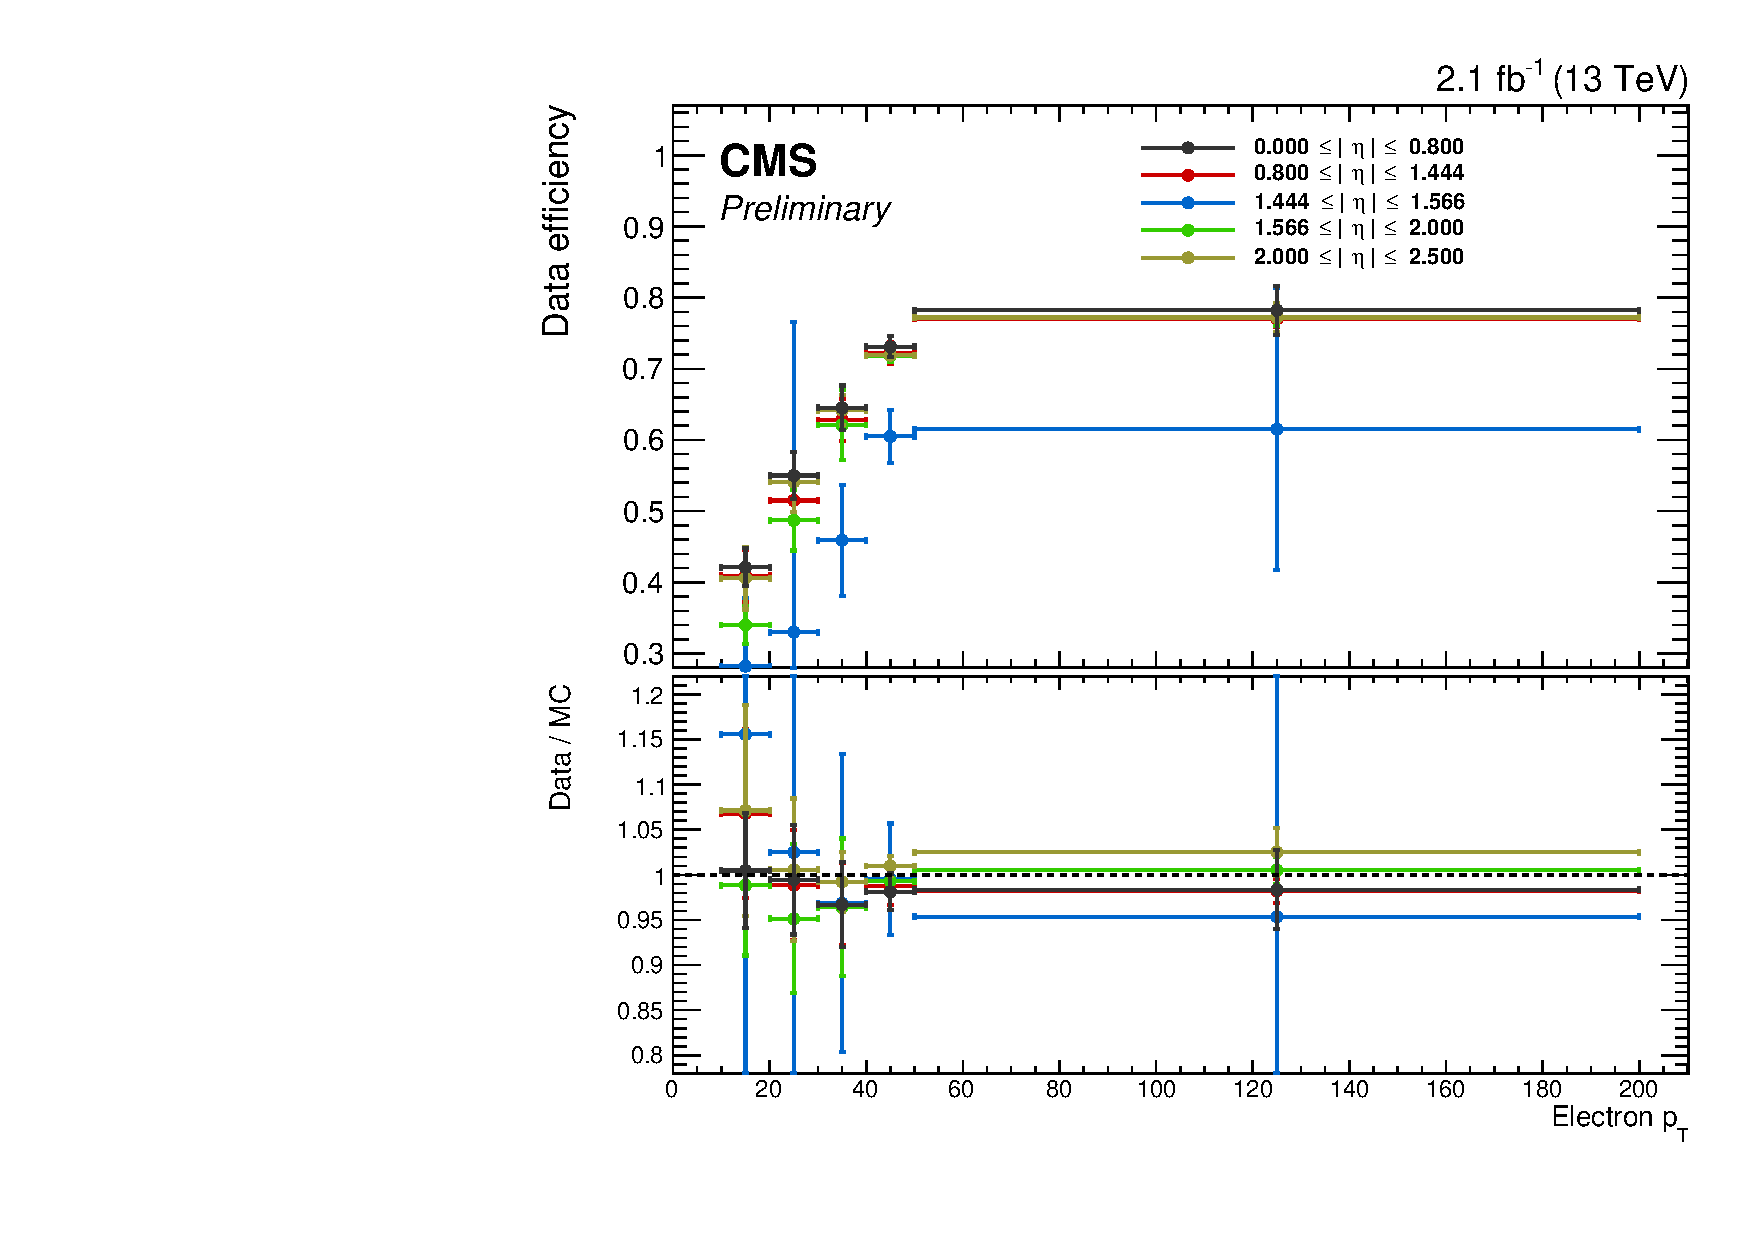
\includegraphics[width=0.5\textwidth]{images/effEleIdIso.pdf}
\caption{Typical electron identification and isolation efficiencies in data (top panel) and data/simulation scale factor (bottom panel), as a function of the electron \pt and for different $\eta$ bins.}\label{fig:eleIdIso}
\end{figure}
	
\subsubsection{Lepton trigger efficiency}\label{sec:trigeff}
Analyses that involves leptons in the final state generally select the interesting events using lepton triggers. For instance, the \hwwllnn channel is characterized by the presence of two leptons in the final state, thereby both single lepton and double lepton triggers are used. The lepton triggers at the HLT level are characterized by \pt thresholds, above which the trigger efficiency is very high (plateau region). Nevertheless, the trigger efficiency as a function of the lepton \pt is not a step function, but is characterized by a steep increase of the efficiency around the \pt threshold (turn-on region). The simulated samples thus need to be corrected in order to properly take into account the trigger efficiency. This can be achieved in two ways: including the HLT trigger in the event simulation or calculating the trigger efficiency in data and then applying it on top of simulated events. Several analyses, such as those related to the \hwwllnn channel, opt for the second approach.

The trigger efficiency for single and double lepton triggers is calculated in bins of $\eta$ and \pt using a Tag and Probe technique similar to the one described in Sec.~\ref{sec:lepIdIsoEff}, separately for muons and electrons. Since the triggered events arise from a mixture of two different triggers, the combined efficiency has to be computed and applied to simulated samples as an event weight. In the following, the approach used in the \hwwllnn analyses is described.

The event efficiency $\varepsilon_\mathrm{ev}$ for an event with two leptons to pass the single lepton trigger is given by the following formula:

\begin{equation}\label{eq:single_trigg}
\varepsilon_\mathrm{ev} = 1 - (1-\varepsilon_{S,\ell1})\cdot(1-\varepsilon_{S,\ell2})\quad,
\end{equation}

where $\varepsilon_{S,\ell1}$ and $\varepsilon_{S,\ell2}$ are the efficiencies for the leading and subleading lepton to pass the single lepton trigger. In other words, the dilepton event passes the single lepton trigger if either one of the two leptons passes the single lepton trigger, excluding the cases for which both leptons pass the trigger. 

For double lepton triggers the efficiency is calculated separately for each leg of the trigger. In the calculation of the efficiencies, the two trigger legs are considered independent, given that the correlations are very small. The combined efficiency is then used as a kinematics-dependent weight to be applied on top of simulated events. The event efficiency can be written as:

\begin{equation}\label{eq:double_trigg}
\varepsilon_\mathrm{ev}  = \varepsilon_{D,\ell1}^\mathrm{lead} \cdot \varepsilon_{D,\ell2}^\mathrm{trail} + (  1 -  \varepsilon_{D,\ell1}^\mathrm{lead} \cdot \varepsilon_{D,\ell2}^\mathrm{trail})\cdot\varepsilon_{D,\ell1}^\mathrm{trail} \cdot \varepsilon_{D,\ell2}^\mathrm{lead} \quad,
\end{equation}

where $\varepsilon_{D,\ell1}^{\mathrm{lead}(trail)}$ is the efficiency of the first lepton to pass the leading (trailing) leg of the double lepton trigger, and $\varepsilon_{D,\ell2}^{\mathrm{lead}(trail)}$ is the efficiency of the second lepton to pass the leading (trailing) leg of the double lepton trigger. The final event efficiency applied to reweight the events in simulation is given by the boolean OR of the event efficiencies corresponding to the single and double lepton triggers, which, using Eqs.~\eqref{eq:single_trigg} and ~\eqref{eq:double_trigg}, can be written as:

\begin{equation}
\begin{split}
\varepsilon_\mathrm{ev} & = 1 - (1-\varepsilon_{S,\ell1})\cdot(1-\varepsilon_{S,\ell2}) + \\
                     & + (1-\varepsilon_{S,\ell1})\cdot(1-\varepsilon_{S,\ell2}) \cdot \\
                     & \cdot [ \varepsilon_{D,\ell1}^\mathrm{lead} \cdot \varepsilon_{D,\ell2}^\mathrm{trail} + (  1 -  \varepsilon_{D,\ell1}^\mathrm{lead} \cdot \varepsilon_{D,\ell2}^\mathrm{trail})\cdot\varepsilon_{D,\ell1}^\mathrm{trail} \cdot \varepsilon_{D,\ell2}^\mathrm{lead} ] \quad.
\end{split}
\end{equation}

%The term that multiplies the double lepton trigger event efficiency is needed to ensure that the events passing the double lepton trigger do not pass also the single lepton trigger.

	
\subsection{Jets reconstruction and identification}\label{chap2:jets}

Jets are the experimental signature of quarks and gluons produced in high energy physics processes. They arise from the hadronization of partons, which forms collimated sprays of particles, and play a predominant role in hadron colliders like the LHC, where the production cross section is very large. In this section, the jet reconstruction techniques used in CMS are described.

\subsubsection{Jet reconstruction in CMS}

The majority of physics analyses involving jets in the final state make use of particle flow jets. The PF jets are reconstructed using the technique described in Sec.~\ref{sec:PF}, clustering all particles reconstructed with the PF algorithm, without any distinction of type and energy threshold. This method allows a remarkable improvement in the jet momentum and spatial resolutions with respect to the calorimeter jets, which are instead reconstructed using solely the information from the calorimeters, as the use of the tracker information provides a better \pt resolution for the charged particles constituting the jets\footnote{On average, the typical jet energy fractions carried by charged particles, photons and neutral particles are 65\%, 25\% and 10\%, respectively.}. 

Jets are defined through sequential, iterative clustering algorithms that combine the four-momenta of input particles until certain conditions are satisfied and jets are formed~\cite{Salam:2009jx}. Several algorithms are available for jet clustering, characterized by different features. From a theoretical point of view, an ideal jet clustering algorithm should fulfil the following requirements~\cite{Blazey:2000qt}:
\begin{itemize}
\item \emph{Infrared safety}: infrared singularities should not appear in the perturbative calculations and the solutions of the algorithm should be insensitive to soft radiation in the event;
\item \emph{Collinear safety}: collinear singularities should not appear in the perturbative calculations and jets should be insensitive to collinear radiation in the event;
\item \emph{Invariance under boosts}: the solutions of the algorithm should be the same independently of boosts in the longitudinal direction. This is particularly important for pp colliders, where the centre-of-mass of the individual proton proton collisions is typically boosted along the beam direction;
\item \emph{Order independence}: the algorithm should find the same jets at parton, particle and detector level;
\item \emph{Straightforward implementation}: the algorithm should be straightforward to implement in perturbative calculations.
\end{itemize}
The ideal algorithm should also follow some experimental attributes. Among them, the performance of the algorithm should be as independent as possible of the detector that provides the data, the algorithm should not amplify the inevitable effects of resolution smearing and angle bias and should not be strongly affected by pile up and high beam luminosities. Furthermore, the algorithm should be easy to implement, efficient to identify all possible jet candidates and should keep at an acceptable level the necessary computing resources.

Two main classes of jet clustering algorithms can be defined. The first one consists in the ``cone'' recombination, where jets are reconstructed associating together particles whose trajectories lie within a cone of radius $\Delta R$ in the $\eta$--$\phi$ plane. The second class of algorithms uses the sequential recombination scheme, that iteratively recombine the closest pair of particles according to some distance measure. The standard algorithms used by CMS are the SISCone, which is a ``cone'' recombination algorithm, and the $k_t$, anti-$k_t$ and \emph{Cambridge Aachen} (CA) algorithms, which instead belong to the sequential recombination class.
All the analyses presented in Secs.~\ref{chap4}, \ref{chap5} and \ref{chap6} make use of the sequential recombination scheme, in particular of the anti-$k_t$ algorithm with $R=0.4$, which is briefly described in the following.

The $k_t$, anti-$k_t$ and CA algorithms are infrared and collinear safe algorithms characterized by the introduction of two definitions of distance: $d_{ij}$, the distance the two objects $i$ and $j$, and $d_{iB}$, the distance between the object $i$ and the beam. These distances are defined by the following equations:
\begin{equation}\label{eq:jetalgo}
\begin{split}
d_{ij} &= min\left(k_{ti}^{2p}, k_{tj}^{2p} \right) \frac{\Delta_{ij}^2}{R^2} \quad,\\
d_{iB} &= k_{ti}^{2p} \quad,
\end{split}
\end{equation}
where $\Delta_{ij} = (y_i - y_j)^2 + (\phi_i - \phi_j)^2$ and $k_ti$, $y_i$ and $\phi_i$ are the transverse momentum, rapidity and azimuthal angle of the particle $i$, respectively. In these formulas, $R$ represents the radial parameter and $p$ is a parameter that is 1 for $k_t$, 0 for CA and $-1$ for anti-$k_t$ algorithm. The algorithm proceeds as follows:
\begin{itemize}
\item the distances $d_{ij}$ are calculated for all pair of particle $i,j$ and the distances $d_{iB}$ are calculated for each particle $i$, according to Eq.~\eqref{eq:jetalgo};
\item the smallest distance, which could be either of type $d_{ij}$ or $d_{iB}$, is identified;
\item if the smallest distance is a $d_{ij}$, the particles $i$ and $j$ are combined into a single new particle summing their four-momenta and the algorithm restarts from the first step;
\item otherwise, if it is a $d_{iB}$, $i$ is declared to be a final state jet and the algorithm returns to the first step;
\item the procedure is repeated until no particles are left.
\end{itemize}

The physical difference between the three algorithms is the momentum weighting. For the $k_t$ algorithm, the weighting proportional to $k_t^2$ implies that jets are reconstructed starting from particles with low transverse momentum. Moreover this algorithm produces jets with irregular borders, thereby complicating the correction for effects such as pile up. For the CA algorithm there is no transverse momentum weighting, and the particles are merged following just an angular approach, based on the distance $\Delta_{ij}$. Also this algorithm leads to jets with irregular borders. Finally, the anti-$k_t$ algorithm, uses a weighting proportional to $1/k_t^2$, favouring the merging of high transverse momentum particles. In this case the jets grow around the particles with highest transverse momenta and the jets have a circular shape. 

Jets reconstructed with different algorithms starting from the same set of simulated particles are shown in Fig.~\ref{fig:jets}.

\begin{figure}[htb]
\centering
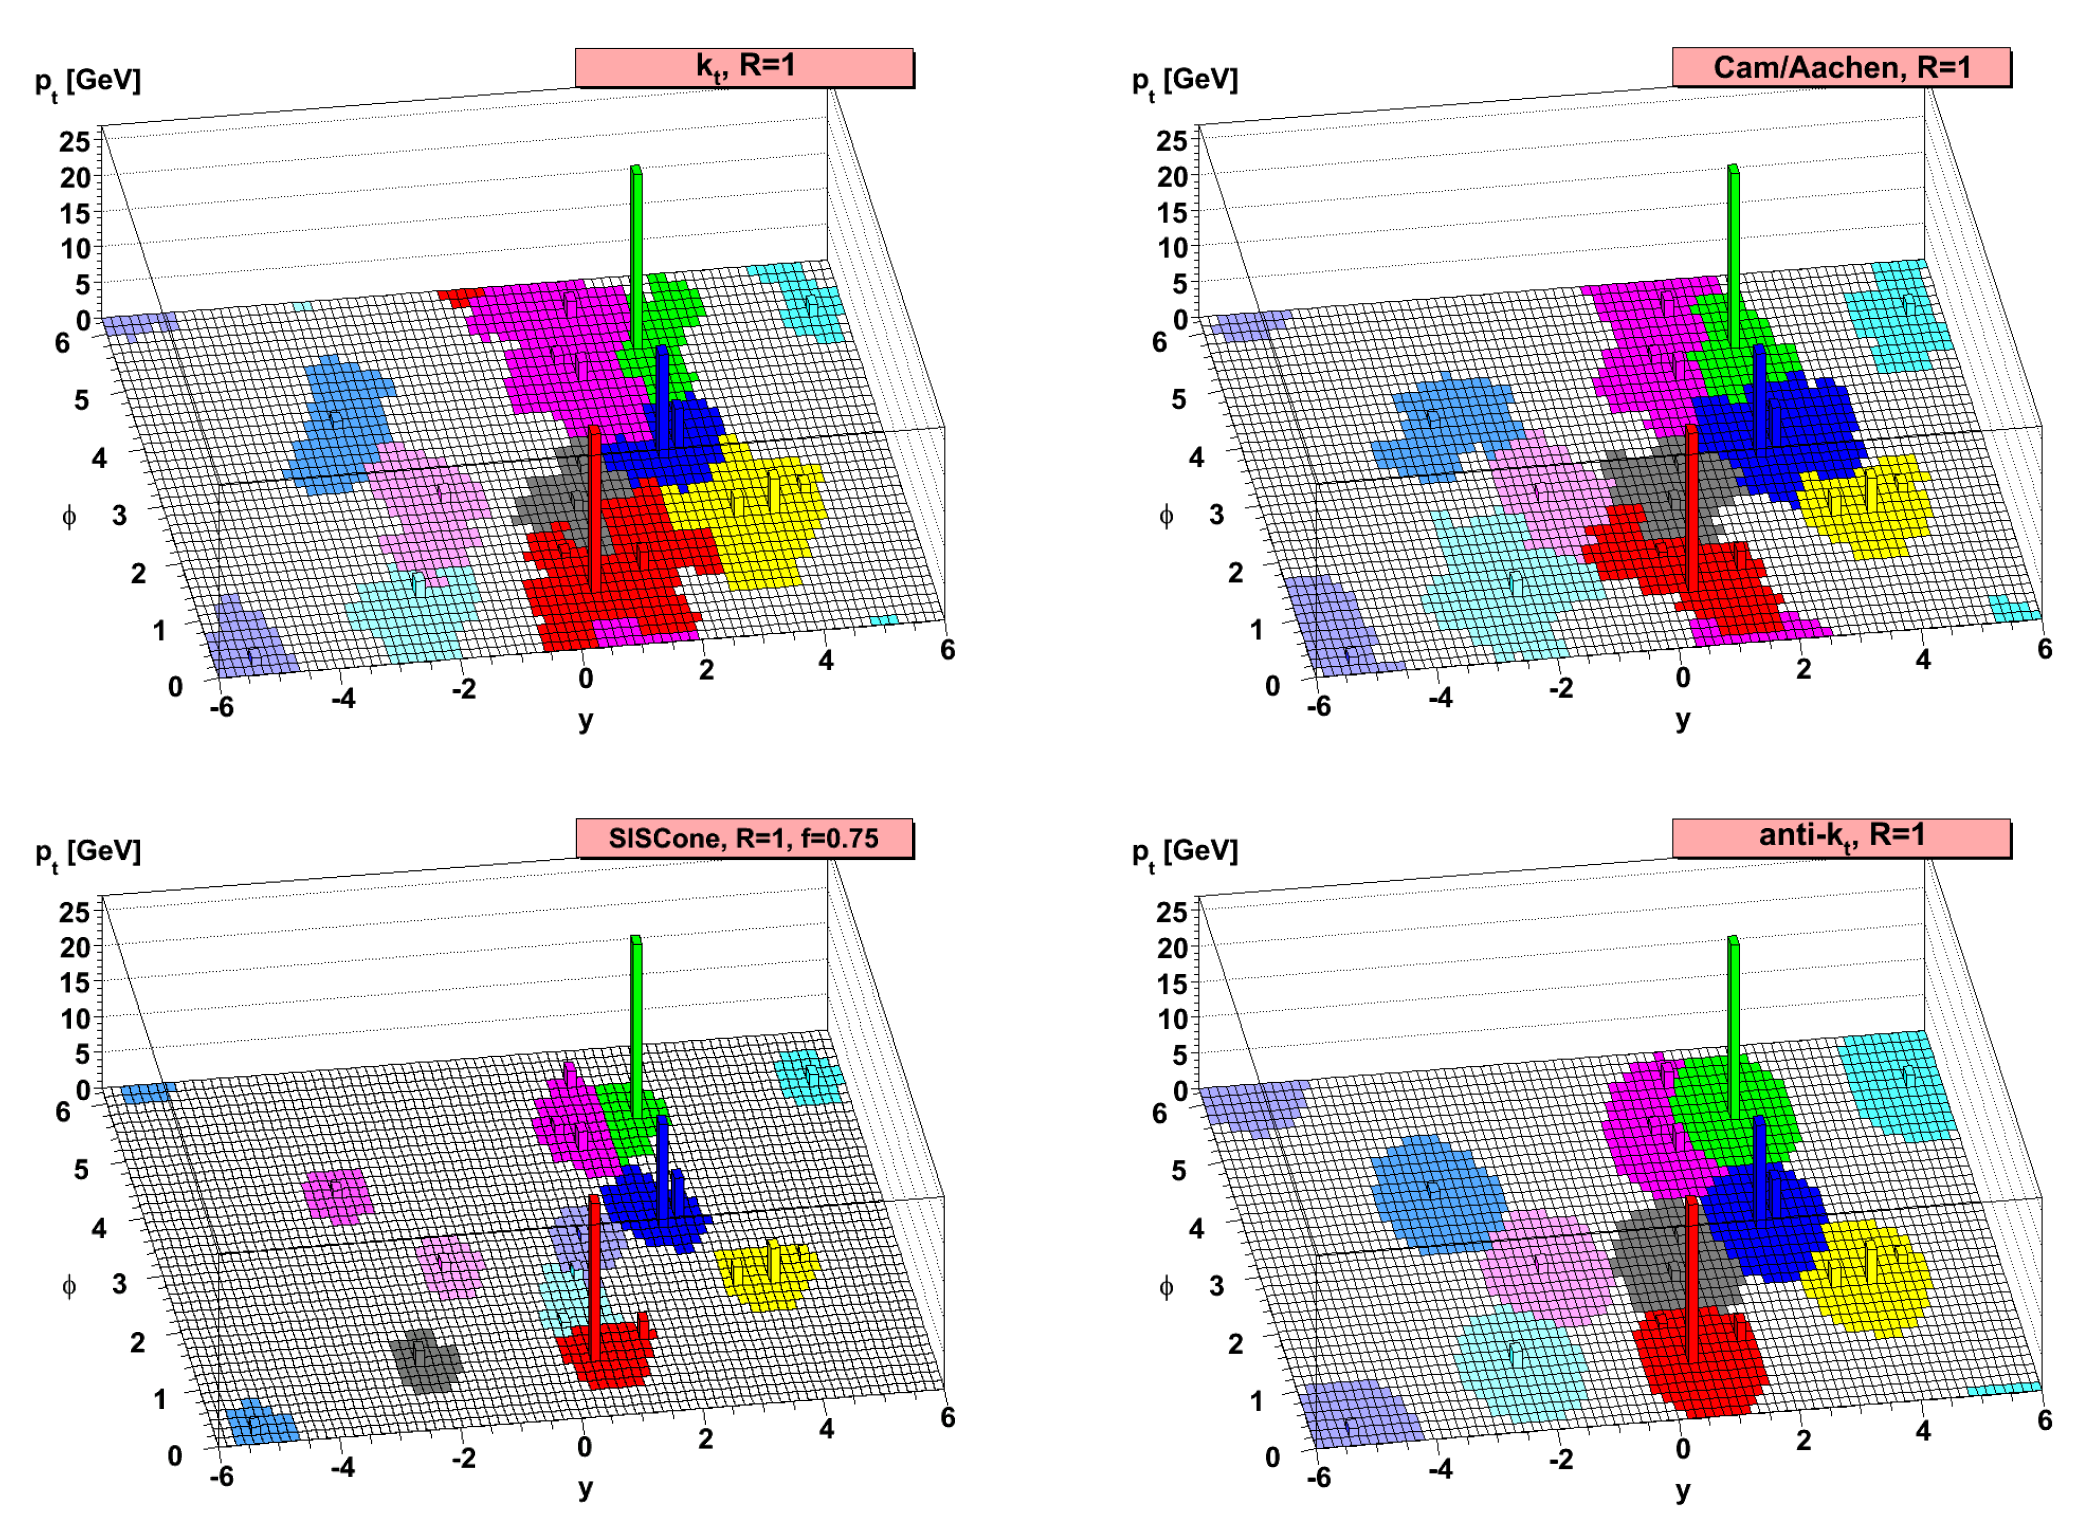
\includegraphics[width=0.7\textwidth]{images/jets.png}
\caption{Jets reconstructed with different algorithms starting from the same set of simulated particles. The jets reconstructed with the sequential recombination algorithms described in the text are shown, as well as with the SISCone algorithm.}\label{fig:jets}
\end{figure}

\subsubsection{Jet energy correction}

The purpose of jet energy correction is to relate, on average, the jet energy measured in the detector to the true energy of the corresponding final state particle or parton jet. The latter is obtained in simulation by clustering, with the same algorithm used for jets in the detector, all the stable particles, i.e. with $c\tau > 1$\,cm, produced in the event excluding neutrinos. This mismatch is mainly ascribable to the non uniform and linear response of the CMS calorimeters, to the electronics noise and to pile up. For this reason, CMS has developed a sequential procedure to calculate and apply the \emph{Jet energy corrections} (JEC)~\cite{Chatrchyan:2011ds}.

The correction is applied as a multiplicative factor $\mathcal{C}$ to each component of the raw jet four-momentum $p_\mu^\mathrm{raw}$ (components are indexed by $\mu$ in the following):
\begin{equation}
p_\mu^\mathrm{cor} = \mathcal{C}\cdot p_\mu^\mathrm{raw} \quad,
\end{equation}
where $p_\mu^\mathrm{cor}$ is the corrected jet four-momentum. The correction factor is composed of the offset correction $C_\mathrm{offset}$, the MC calibration factor $C_\mathrm{MC}$, and the residual calibrations $C_\mathrm{rel}$ and $C_\mathrm{abs}$ for the relative and absolute energy scales, respectively. The offset correction removes the extra energy due to noise and pile up, and the MC correction removes the bulk of the non-uniformity in $\eta$ and the non-linearity in \pt. Finally, the residual corrections account for the small differences between data and simulation.  The various components are applied in sequence as described by the equation below:
\begin{equation}
\mathcal{C} = C_\mathrm{offset}(\pt^\mathrm{raw}) \cdot C_\mathrm{MC}(\pt',\eta) \cdot C_\mathrm{rel}(\eta) \cdot C_\mathrm{abs}(\pt'') \quad ,
\end{equation}
where $\pt'$ is the jet \pt after applying the offset correction and $\pt''$ is the jet \pt after applying all previous corrections. Each component is briefly described in the following sections.

\subsubsubsection{Offset correction}
 
The offset correction purpose is to estimate and subtract, on average, the energy contribution that is not associated with the hard scattering in the event. The energy excess includes contributions from electronics noise and pile up.

\subsubsection{Jet b tagging}










	
